% !TeX program = lualatex
% !TeX root = ../../main.tex
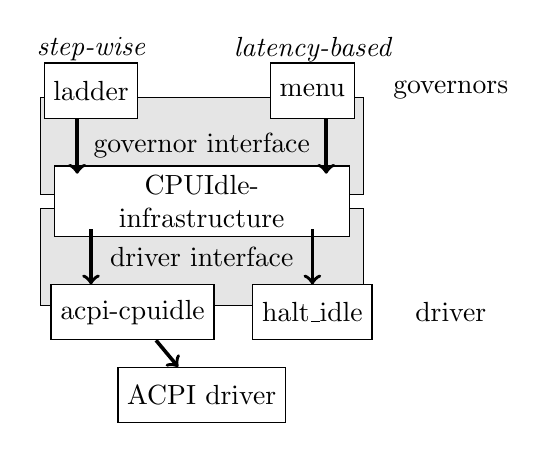
\begin{tikzpicture}[every node/.style={text centered}]
		\draw (0em, -2em)		node[draw, fill=gray!20%]
, text width=11em, minimum height=3.5em]
				{driver interface}

			(0em, 2em)		node[draw, fill=gray!20%]
, text width=11em, minimum height=3.5em]
				{governor interface}

			(0em, 0em)		node[draw, fill=white%]
, text width=10em, minimum height=2em] (cpuidle)
				{CPUIdle-infrastructure}



			(-4em, 4em)		node[draw, fill=white%]
, minimum height=2em] (ladder)
				{ladder}			
			(-4em, 5.5em)	node[font=\itshape] {step-wise}


			(4em, 4em)		node[draw, fill=white%]
, minimum height=2em] (menu)
				{menu}			
			(4em, 5.5em)	node[font=\itshape] {latency-based}




			(9em, 4em)	node {governors}
			(9em, -4em)	node {driver}
			
			(-2.5em, -4em)	node[draw%]
, minimum height=2em, fill=white] (acpiidle)
				{acpi-cpuidle}




			(0em, -7em)	node[draw%]
, minimum height=2em, fill=white] (acpidriver)
				{ACPI driver}

			(4em, -4em)	node[draw%]
, minimum height=2em, fill=white] (haltidle)
				{halt\_idle}
;

	\draw[->, line width=1.3pt] (4.5em, 3em) -- (4.5em, 1em);%(menu) -- (cpuidle);
	\draw[->, line width=1.3pt] (-4.5em, 3em) -- (-4.5em, 1em);%(ladder) -- (cpuidle);

	\draw[<-, line width=1.3pt] (4em, -3em) -- (4em, -1em);%(haltidle) -- (cpuidle);
	\draw[<-, line width=1.3pt] (-4em, -3em) -- (-4em, -1em);%(acpiidle) -- (cpuidle);
	\draw[<-, line width=1.3pt] (acpidriver) -- (acpiidle);
\end{tikzpicture}